\section{Introduction}

\subsection{Motivation}
Nowadays a car is full of small computers handling tasks for the whole system. Without these helpers, functions like driver-assistance or self-diagnostic would not be possible. Those computers are generally called electronic control unit (ECU). Modern cars can contain over 100 of those. The complexity of ECU networks in a car is increasing quickly. The next generation of car networks is expected to be more centralized with less ECUs \cite{car-architecture}. This reduces complexity and its inherent risk of security vulnerabilities and high costs, as shown in \autoref{fig:centralized-architecture}.

%durations
\begin{figure}[h]
    \centering
    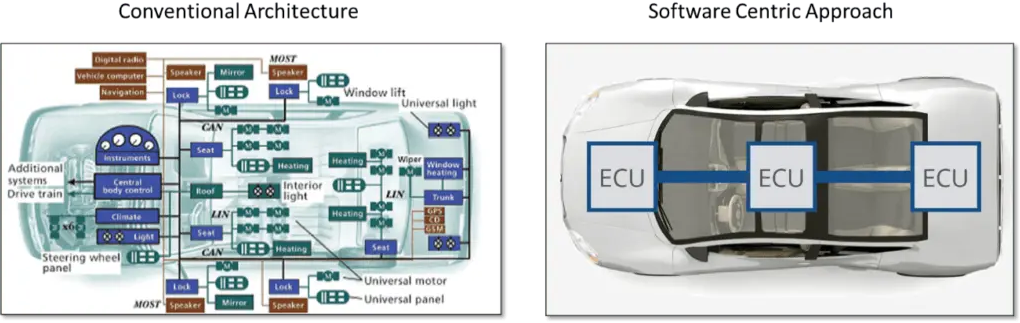
\includegraphics[width=1\textwidth]{centralized-architecture}
    \caption{Illustration of the current and the next-gen architecture of cars \cite{car-architecture}.}
    \label{fig:centralized-architecture}
\end{figure}

ECUs communicate with each other via bus systems. The most common ones are CAN, FlexRay and the Automotive Ethernet, which is becoming increasingly popular. Transport protocols usually sit on top of these physical layers. For Ethernet this is the well known TCP protocol, while the most common one for CAN is the ISO-TP protocol. Application protocols are used to ultimately transfer payload. For example, some protocols were created specifically for the development of units like Universal Measurement and Calibration Protocol (XCP) and some others were defined for diagnostic purposes such as Unified Diagnostic Services (UDS), General Motors Local Area Network (GMLAN) and On-board diagnostics (OBD). Both types are security critical. The XCP protocol is able to read and even write into the flash memory of an ECU. It shall be disabled on shipped ECUs. The UDS and GMLAN protocol provide definitions for diagnostic related tasks. However, diagnostic protocols are explicitly designed for actively used cars and thus exposed to the easily accessible OBD-II port, which by regulation must be present near the steering wheel on at least every car built after 2003 (see \autoref{fig:obd-port}). This fact makes them a great first target for gathering information. This work puts the UDS protocol in focus since it is the widest adopted protocol which allows extended functionality, for example flashing ECUs. The OBD protocol is excluded in this work because it does not offer any valuable information and the GMLAN protocol because it is restricted to vehicles from the General Motors corporation.

\begin{figure}[h]
    \centering
    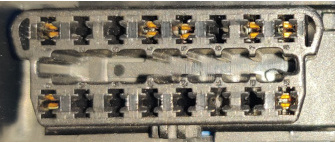
\includegraphics[width=0.5\textwidth]{obd-port}
    \caption{The OBD-II port of a BMW.}
    \label{fig:obd-port}
\end{figure}

The initial step in testing a system for weaknesses is to gather as much information from it as possible. In most cases, a protocol definition does not require that its specifications is fully supported; instead, a subset is sufficient.
Furthermore, a diagnostic protocol can define various states. The ECU may show varying behaviors in different states, for example support for other services. Since this kind of information is highly relevant for the security of the ECU, it would be helpful for security testers to gain this knowledge quickly and automatically.

One option to achieve this is to send all possible requests to an ECU and evaluate the responses. In the context of the project \emph{Penetration Test Driven Safety and Security System Improvements for Cyber-Critical Systems} (PetS3) \cite{pets3} such scanners have been implemented for UDS, GMLAN and OBD.

With their brute-force approaches, they are effective but not efficient. A scan can take a highly variable amount of time. It can range from a few hours to a day or more. In general, the more states are found on an ECU in a scan, the more time it will need. For example, more authentication information leads to more state detections and thus to higher runtimes. In addition, the response time of the ECU is also a decisive factor. The original runtimes observed of one UDS scan on the available ECUs are shown in \autoref{fig:durations} generated with the \mintinline{text}{plotly} library \cite{plotly}. It should be noted, that these scans have been executed with no additional information about the ECU as well. Accordingly, only the states that can be found without further information were detected.

%durations
\begin{figure}[h]
    \centering
    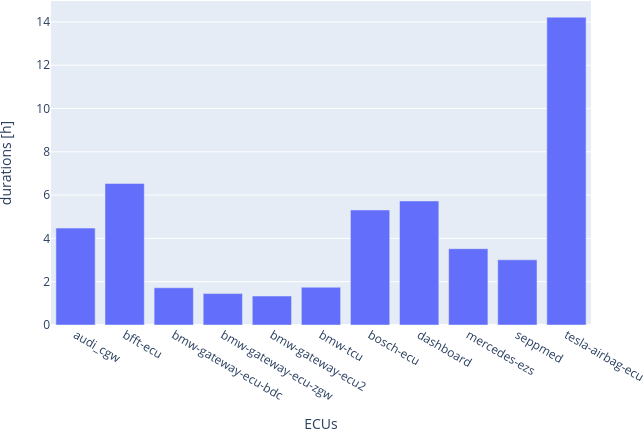
\includegraphics[width=1\textwidth]{durations}
    \caption{Observed runtimes for one UDS scan.}
    \label{fig:durations}
\end{figure}

Consequently, an efficient scan is desirable that keeps the scan time low even though many states can be found or the ECU has a high response time.

\subsection{Goal}

This paper evaluates different approaches to improve the efficiency of the UDS protocol scanning. The approaches can be mixed freely, if this leads to better results.

Efficiency improvement is understood as the ratio between the speed-up and the coverage. Coverage is here defined as the ratio of finds in the unmodified Scanner to the finds of the modified Scanner, and the speed-up as the saved time in comparison between these two. For both metrics, the higher the better.

Nevertheless, the coverage and speed-up have to be in balance. A speed-up of 90\% is not helpful if this results in 0\% coverage. The speed-up is achieved by reducing the number of generated packets. Hence, the challenge is to narrow down the scanning area to where positive responses are expected.


\subsection{Environment}
This work was created at eMundo GmbH in Ingolstadt. It is an IT service company which plans and executes projects for customers. Also, it is an aspiring company which in 20 years managed to open in total six company headquarters in Germany, Austria and Italy with almost 100 employees.

Since 2018, they are part of the \emph{Penetration Test Driven Safety and Security System Improvements for Cyber-Critical Systems} (PetS3) project. It is a collaboration research project among the OTH Regensburg, TH Nürnberg, EDAG Engineering Group AG, sepp.med GmbH, intive automotive GmbH and eMundo GmbH.

Due to the advancing networking, cyberattacks are a growing threat to a variety of application areas such as connected vehicles or smart metering. Common concepts of functional safety and IT security are required for these gateway-based systems. The aim of the research project is to investigate attacks on the IT security of system architectures of networked cyber-critical systems, since the interaction between functional safety and IT security is largely unknown in this context.

This paper is the final result of this project on the part of eMundo.

\subsection{Outline}
